\documentclass[tikz,border=6pt]{standalone}

\usepackage{amsmath}
\usepackage{xcolor}
\usetikzlibrary{arrows.meta,calc}

\definecolor{passivebg}{HTML}{EEF5FC}
\definecolor{passivebox}{HTML}{D9EBFA}
\definecolor{activebg}{HTML}{F0F8EF}
\definecolor{activebox}{HTML}{DFF1DF}
\definecolor{pqbox}{HTML}{FFF2C4}
\definecolor{txbox}{HTML}{FFE2B8}
\definecolor{attackbg}{HTML}{FFF1EF}
\definecolor{attackbox}{HTML}{FFD8D0}
\definecolor{edge}{HTML}{343F49}
\definecolor{boundary}{HTML}{7A4B15}
\definecolor{gradblue}{HTML}{2F63B8}
\definecolor{attackred}{HTML}{A43D2F}

\begin{document}
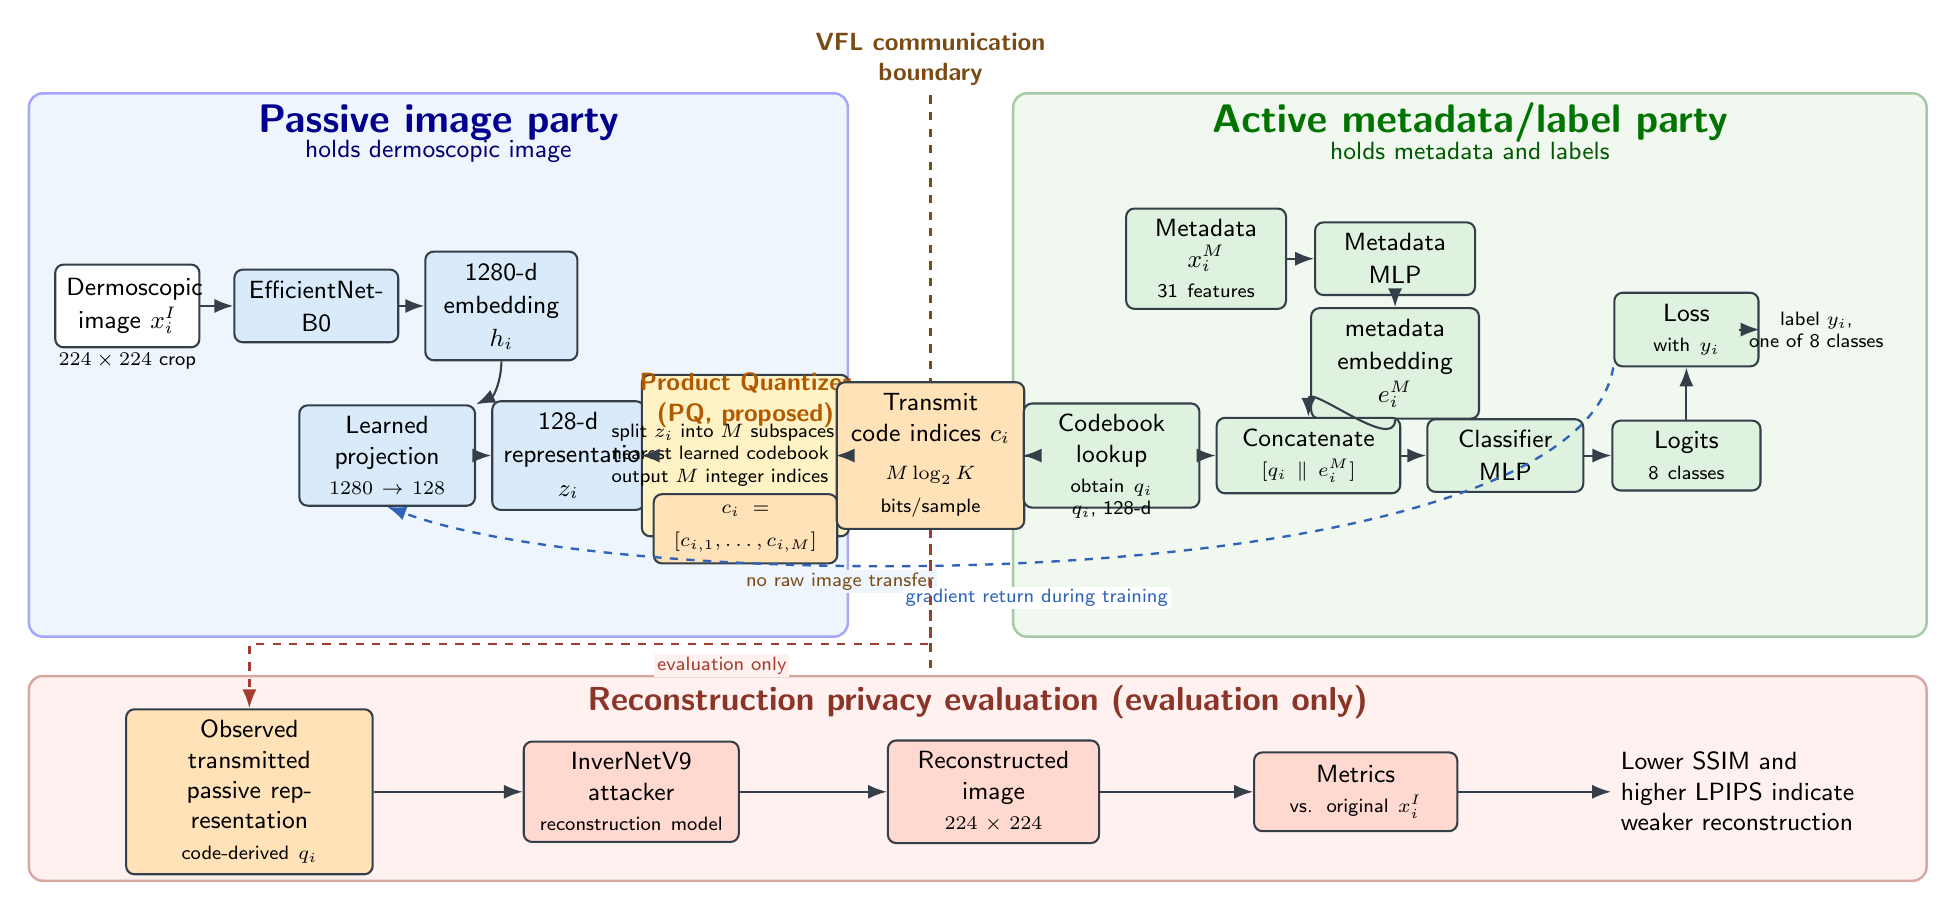
\begin{tikzpicture}[
    font=\sffamily,
    >=Latex,
    mainarrow/.style={-{Latex[length=2.4mm]}, draw=edge, line width=0.75pt},
    gradarrow/.style={-{Latex[length=2.4mm]}, draw=gradblue, dashed, line width=0.85pt},
    attackarrow/.style={-{Latex[length=2.4mm]}, draw=attackred, dashed, line width=0.85pt},
    box/.style={
        rounded corners=3pt,
        draw=edge,
        line width=0.75pt,
        align=center,
        inner sep=4pt,
        minimum height=0.85cm
    },
    title/.style={font=\sffamily\bfseries\Large},
    subtitle/.style={font=\sffamily\small},
    small/.style={font=\sffamily\small},
    tinytext/.style={font=\sffamily\scriptsize}
]

% ---------------------------------------------------------------------
% Canvas regions.
% ---------------------------------------------------------------------
\filldraw[fill=passivebg, draw=blue!35, line width=0.9pt, rounded corners=5pt]
    (0.3,3.25) rectangle (10.7,10.15);
\filldraw[fill=activebg, draw=green!40!black!35, line width=0.9pt, rounded corners=5pt]
    (12.8,3.25) rectangle (24.4,10.15);
\filldraw[fill=attackbg, draw=attackred!45, line width=0.9pt, rounded corners=5pt]
    (0.3,0.15) rectangle (24.4,2.75);

\node[title, text=blue!55!black] at (5.5,9.78) {Passive image party};
\node[subtitle, text=blue!45!black] at (5.5,9.42) {holds dermoscopic image};
\node[title, text=green!45!black] at (18.6,9.78) {Active metadata/label party};
\node[subtitle, text=green!35!black] at (18.6,9.42) {holds metadata and labels};
\node[font=\sffamily\bfseries\large, text=attackred!85!black] at (12.35,2.42)
    {Reconstruction privacy evaluation (evaluation only)};

% Boundary is drawn first so filled boxes cover it where necessary.
\draw[dashed, draw=boundary, line width=1.0pt] (11.75,2.85) -- (11.75,10.32);
\node[font=\sffamily\bfseries\small, text=boundary, align=center, fill=white, inner sep=2pt]
    at (11.75,10.58) {VFL communication\\boundary};

% ---------------------------------------------------------------------
% Passive image party.
% ---------------------------------------------------------------------
\node[box, fill=white, text width=1.55cm, minimum height=1.05cm] (img) at (1.55,7.45)
    {\small Dermoscopic\\image $x_i^I$};
\node[tinytext] at (1.55,6.75) {$224\times224$ crop};

\node[box, fill=passivebox, text width=1.80cm] (eff) at (3.95,7.45)
    {\small EfficientNet-B0};
\node[box, fill=passivebox, text width=1.65cm] (h) at (6.30,7.45)
    {\small 1280-d\\embedding $h_i$};

\node[box, fill=passivebox, text width=1.95cm] (proj) at (4.85,5.55)
    {\small Learned projection\\[-1pt]\scriptsize $1280\to128$};
\node[box, fill=passivebox, text width=1.65cm] (z) at (7.15,5.55)
    {\small 128-d\\representation $z_i$};

\node[box, fill=pqbox, text width=2.35cm, minimum height=2.05cm] (pq) at (9.40,5.55) {};
\node[font=\sffamily\bfseries\small, text=orange!70!black, align=center] at (9.40,6.25)
    {Product Quantizer\\(PQ, proposed)};
\node[font=\sffamily\scriptsize, align=left] at (9.40,5.55)
    {\begin{tabular}{@{}l@{}}
    split $z_i$ into $M$ subspaces\\
    nearest learned codebook entry\\
    output $M$ integer indices
    \end{tabular}};
\node[box, fill=txbox, text width=2.05cm, minimum height=0.58cm] (ci) at (9.40,4.62)
    {\scriptsize $c_i=[c_{i,1},\ldots,c_{i,M}]$};

\draw[mainarrow] (img) -- (eff);
\draw[mainarrow] (eff) -- (h);
\draw[mainarrow] (h.south) to[out=-90,in=25] (proj.north east);
\draw[mainarrow] (proj) -- (z);
\draw[mainarrow] (z) -- (pq.west);

% One clean transmission object at the boundary.
\node[box, fill=txbox, text width=2.10cm, minimum height=1.22cm] (tx) at (11.75,5.55)
    {\small Transmit\\code indices $c_i$\\[2pt]
    \scriptsize $M\log_2K$ bits/sample};
\draw[mainarrow] (pq.east) -- (tx.west);
\node[tinytext, text=boundary, fill=passivebg, inner sep=1pt] at (10.60,3.95) {no raw image transfer};

% ---------------------------------------------------------------------
% Active metadata/label party.
% ---------------------------------------------------------------------
\node[box, fill=activebox, text width=1.95cm] (lookup) at (14.05,5.55)
    {\small Codebook lookup\\[-1pt]\scriptsize obtain $q_i$};
\node[tinytext] at (14.05,4.86) {$q_i$, 128-d};
\draw[mainarrow] (tx.east) -- (lookup.west);

\node[box, fill=activebox, text width=1.75cm] (meta) at (15.25,8.05)
    {\small Metadata $x_i^M$\\[-1pt]\scriptsize 31 features};
\node[box, fill=activebox, text width=1.75cm] (metamlp) at (17.65,8.05)
    {\small Metadata MLP};
\node[box, fill=activebox, text width=1.85cm] (emb) at (17.65,6.72)
    {\small metadata\\embedding $e_i^M$};
\node[box, fill=activebox, text width=2.05cm] (concat) at (16.55,5.55)
    {\small Concatenate\\[-1pt]\scriptsize $[q_i \parallel e_i^M]$};
\node[box, fill=activebox, text width=1.70cm] (clf) at (19.05,5.55)
    {\small Classifier\\MLP};
\node[box, fill=activebox, text width=1.60cm] (logits) at (21.35,5.55)
    {\small Logits\\[-1pt]\scriptsize 8 classes};
\node[box, fill=activebox, text width=1.55cm] (loss) at (21.35,7.15)
    {\small Loss\\[-1pt]\scriptsize with $y_i$};
\node[tinytext, align=center] (label) at (23.00,7.15)
    {label $y_i$,\\one of 8 classes};

\draw[mainarrow] (meta) -- (metamlp);
\draw[mainarrow] (metamlp) -- (emb);
\draw[mainarrow] (lookup) -- (concat);
\draw[mainarrow] (emb.south) to[out=-90,in=90] (concat.north);
\draw[mainarrow] (concat) -- (clf);
\draw[mainarrow] (clf) -- (logits);
\draw[mainarrow] (logits.north) -- (loss.south);
\draw[mainarrow] (label.west) -- (loss.east);

% Gradient return, routed through the empty band between architecture and evaluation.
\draw[gradarrow] (loss.south west) .. controls (19.9,3.72) and (8.0,3.72) .. (proj.south);
\node[font=\sffamily\scriptsize, text=gradblue, fill=white, inner sep=1pt]
    at (13.10,3.74) {gradient return during training};

% ---------------------------------------------------------------------
% Reconstruction privacy evaluation.
% ---------------------------------------------------------------------
\node[box, fill=txbox, text width=2.85cm, minimum height=1.08cm] (obs) at (3.10,1.28)
    {\small Observed transmitted\\passive representation\\[-1pt]
    \scriptsize code-derived $q_i$};
\node[box, fill=attackbox, text width=2.45cm, minimum height=1.00cm] (inv) at (7.95,1.28)
    {\small InverNetV9 attacker\\[-1pt]\scriptsize reconstruction model};
\node[box, fill=attackbox, text width=2.40cm, minimum height=1.00cm] (recon) at (12.55,1.28)
    {\small Reconstructed image\\[-1pt]\scriptsize $224\times224$};
\node[box, fill=attackbox, text width=2.30cm, minimum height=1.00cm] (metrics) at (17.15,1.28)
    {\small Metrics\\[-1pt]\scriptsize vs. original $x_i^I$};
\node[font=\sffamily\small, align=left] (privacy) at (22.00,1.28)
    {Lower SSIM and\\higher LPIPS indicate\\weaker reconstruction};

\draw[attackarrow] (tx.south) -- ++(0,-1.45) -| (obs.north);
\node[font=\sffamily\scriptsize, text=attackred, fill=attackbg, inner sep=1pt]
    at (9.10,2.88) {evaluation only};
\draw[mainarrow] (obs) -- (inv);
\draw[mainarrow] (inv) -- (recon);
\draw[mainarrow] (recon) -- (metrics);
\draw[mainarrow] (metrics) -- (privacy.west);

\end{tikzpicture}
\end{document}
